\section{Contraste de Resultados: Método Exacto vs.\ Metaheurística}\label{sec:contraste}

Esta sección contrasta explícitamente los resultados de las dos soluciones algorítmicas implementadas para el MCP: el modelo ILP resuelto por Ramificación y Acotamiento del Informe~1, y la Búsqueda Tabú con reinicio de este informe.

\subsection{Fuentes de comparación}

Para \textit{keller4} se usa directamente el resultado reportado en el Informe~1: modelo ILP (Pyomo) resuelto con HiGHS, que certificó $\omega=11$ en 12--18\,s. Para \textit{C125.9} no se reportó un resultado formal en el Informe~1 (que se centró en \textit{keller4}); se utiliza en su lugar un experimento exploratorio realizado durante el desarrollo de dicho informe con un Branch \& Bound manual (framework PyBnB \parencite{pybnb}) sobre la relajación LP, ejecutado con un límite de 300\,s. Este experimento es la referencia exacta más directa disponible sobre una instancia más densa que \textit{keller4}, y se documenta aquí junto con sus resultados para dejar la comparación completamente trazable. El notebook ejecutable con el código y las salidas completas de este experimento (incluyendo los 232\,953 nodos explorados y el estado \textit{feasible} final) está disponible en el repositorio del proyecto, en \texttt{notebook/maximum\_clique\_bb.ipynb}.

\paragraph{Nota metodológica sobre las dos referencias exactas.} Ambas referencias exactas no son metodológicamente idénticas entre sí, lo cual es relevante para interpretar el contraste. HiGHS es un solver MIP industrial que, internamente, combina la Ramificación y Acotamiento con planos de corte y heurísticas de factibilidad (Informe~1, Sección~3.2); su tiempo de 12--18\,s en \textit{keller4} refleja, por tanto, un B\&B \emph{asistido por heurísticas}, no una Ramificación y Acotamiento pura. El B\&B manual usado como referencia en \textit{C125.9}, en cambio, sí corresponde a una Ramificación y Acotamiento sin heurísticas ni cortes adicionales: en cada nodo se resuelve únicamente la relajación LP (mediante \texttt{scipy}) y se ramifica sobre una variable fraccionaria, sin mecanismos de aceleración adicionales. Esta segunda referencia es, en consecuencia, la comparación más limpia entre búsqueda exacta pura y metaheurística de las dos presentadas en esta sección. Asimismo, a diferencia del Informe~1 —que evaluó una única instancia—, este informe contrasta ambos enfoques sobre dos instancias de tamaño y densidad distintos (171 vs.\ 125 vértices; densidad 0.65 vs.\ 0.90), lo que permite observar cómo se comporta cada método al variar la dificultad de la instancia y no solo su tamaño nominal.

\subsection{Tabla comparativa}

La Tabla~\ref{tab:contraste} resume ambos enfoques sobre las dos instancias.

\begin{table}[H]
\centering
\small
\caption{Contraste entre el método exacto (Informe 1) y la metaheurística (Informe 2).}
\label{tab:contraste}
\begin{tabularx}{\textwidth}{@{}l X r r c X@{}}
\hline
\textbf{Inst.} & \textbf{Método} & \textbf{$\omega$} & \textbf{Tiempo} & \textbf{¿Óptimo?} & \textbf{Notas} \\
\hline
\multirow{2}{*}{keller4} & ILP + HiGHS (Informe 1) & 11 & 12--18\,s & Sí & Único resultado reportado \\
 & Tabú + ILS (Informe 2) & 11 & 0.021\,s & No & Media 10.90; 28/30 corridas óptimas \\
\hline
\multirow{2}{*}{C125.9} & B\&B manual, PyBnB & 34 & 300\,s (\textit{timeout}) & No & 232\,953 nodos explorados \\
 & Tabú + ILS (Informe 2) & 34 & 0.025\,s & No & Media 33.97; 29/30 corridas óptimas \\
\hline
\end{tabularx}
\end{table}

\begin{figure}[H]
\centering
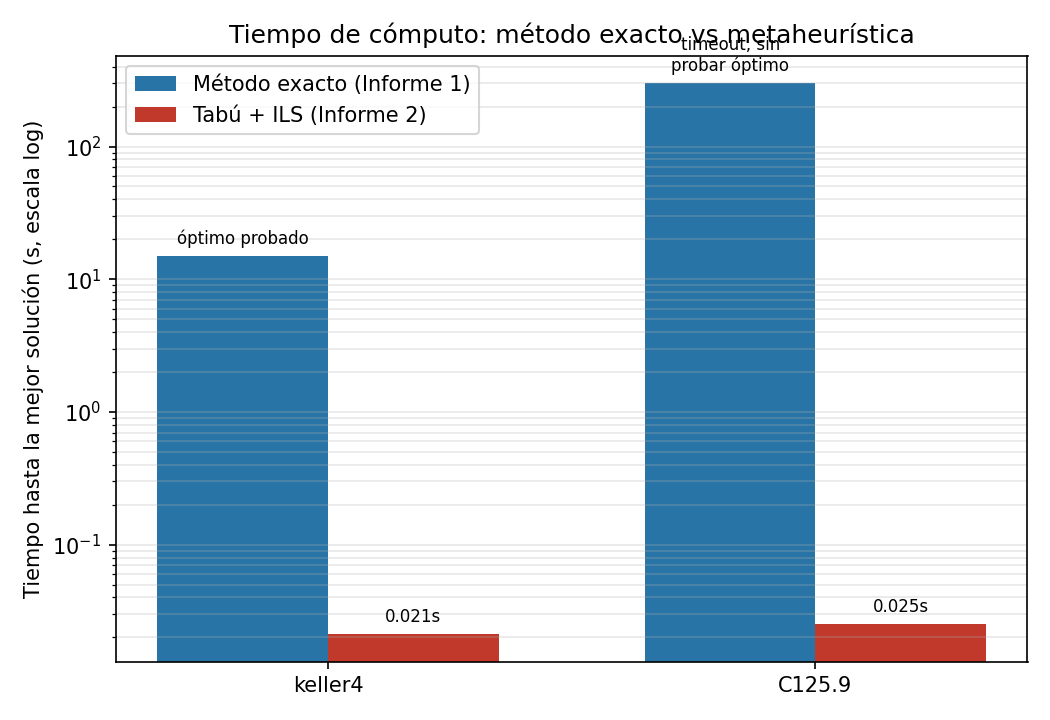
\includegraphics[width=0.75\textwidth]{../notebook_metaheuristica/comparacion_tiempos.png}
\caption{Tiempo hasta la mejor solución: método exacto vs.\ metaheurística (escala logarítmica).}
\label{fig:comparacion_tiempos}
\end{figure}

\FloatBarrier

\subsection{Análisis del contraste}

\paragraph{Calidad de la solución.} En ambas instancias, la mejor solución encontrada por la metaheurística en al menos una corrida coincide exactamente con la del método exacto ($\omega=11$ y $\omega=34$, respectivamente). Considerando el conjunto de las 30 corridas, la calidad media se mantiene muy cercana al óptimo (a 0.10 y 0.03 vértices de distancia en promedio, respectivamente), lo que indica que incluso en las corridas que no alcanzan el óptimo, la solución obtenida es prácticamente óptima en términos prácticos.

\paragraph{Tiempo de cómputo.} La diferencia de tiempos es de varios órdenes de magnitud. En \textit{keller4}, la metaheurística encuentra su mejor solución, en promedio, cerca de 711 veces más rápido que el tiempo que HiGHS tarda en \emph{certificar} el óptimo (0.021\,s vs.\ 15\,s, tomando el punto medio del rango reportado). En \textit{C125.9} la brecha es aún mayor: el B\&B manual agota los 300\,s sin certificar optimalidad, mientras que la metaheurística encuentra su mejor solución en 0.025\,s en promedio —más de 11\,900 veces más rápido—, aunque, a diferencia del caso anterior, ninguno de los dos métodos certifica formalmente que 34 sea el óptimo en esta comparación (el valor $\omega=34$ se toma como óptimo conocido de la instancia según el benchmark DIMACS \parencite{mascia_dimacs}, no como algo demostrado por ninguno de los dos algoritmos aquí ejecutados).

\paragraph{El compromiso central: garantía vs.\ escalabilidad.} El contraste evidencia el trade-off fundamental entre ambos paradigmas, ya anticipado en la introducción de este informe. El método exacto ofrece una \emph{garantía}: cuando termina con estado \textit{óptimo}, no existe clique más grande en el grafo. Esa garantía tiene un costo computacional que crece de forma no controlada con la dificultad de la instancia —en \textit{keller4} son segundos, pero en \textit{C125.9}, con una densidad considerablemente mayor (0.90 vs.\ 0.65) y menos vértices, el mismo tipo de método ya no logra concluir en 300\,s—. La metaheurística invierte esta relación: no ofrece garantía de optimalidad en ninguna corrida individual, pero su tiempo de cómputo es prácticamente insensible a la dificultad de la instancia (0.021\,s y 0.025\,s son estadísticamente indistinguibles pese a que \textit{C125.9} es la instancia donde el método exacto colapsa). La garantía perdida se recupera parcialmente mediante repetición: al ejecutar múltiples corridas independientes y quedarse con la mejor, la probabilidad empírica de \emph{no} encontrar el óptimo cae rápidamente (con una tasa de éxito por corrida de 93--97\,\%, y suponiendo corridas independientes, la probabilidad de que las 30 corridas fallen simultáneamente es inferior a $10^{-30}$).

\paragraph{Cuándo preferir cada enfoque.} A la luz de estos resultados, el método exacto resulta preferible cuando se requiere una garantía formal de optimalidad y la instancia es lo suficientemente pequeña o estructurada para que el árbol de Branch \& Bound sea manejable (como \textit{keller4}). La metaheurística resulta preferible cuando el tiempo de respuesta es crítico, quiere explorarse un gran número de instancias, o la instancia es lo suficientemente grande o densa para que el enfoque exacto sea inviable en la práctica —exactamente el escenario ilustrado por \textit{C125.9}—, aceptando a cambio una solución sin certificado formal de optimalidad, aunque empíricamente de calidad prácticamente óptima.
